
%(BEGIN_QUESTION)
% Copyright 2010, Tony R. Kuphaldt, released under the Creative Commons Attribution License (v 1.0)
% This means you may do almost anything with this work of mine, so long as you give me proper credit

Anta at denne temperaturmålekretsen feilaktig viser svært høy temperatur (fullt utslag) når RTD-sensoren faktisk måler romtemperatur (20 $^{o}$C).  Et digitalt multimeter (DMM) koblet mellom testpunktene {\bf C} og {\bf D} viser 14.99 volt:

$$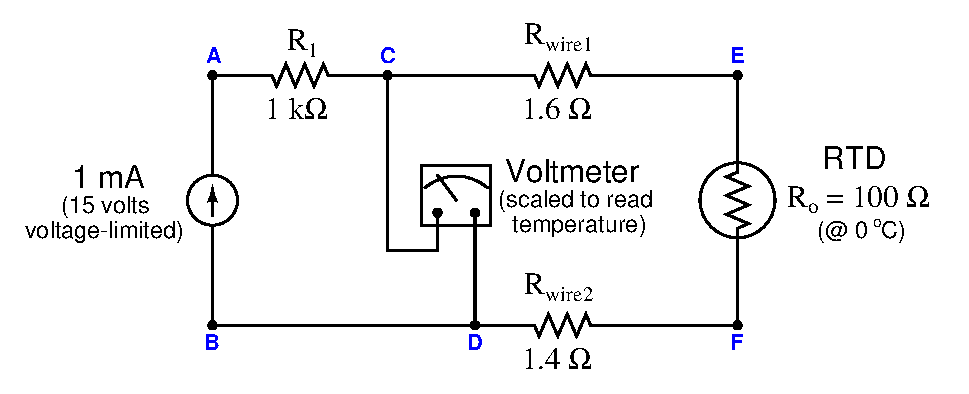
\includegraphics[width=15.5cm]{i00206x01.eps}$$

Vurder sannsynligheten for hver oppgitt feil i denne kretsen.  Vurder en og en feil (ingen samtidige feil), og avgjør om hver feil alene kan forklare \textit{alle} målinger og symptomer i kretsen.

% No blank lines allowed between lines of an \halign structure!
% I use comments (%) instead, so that TeX doesn't choke.

$$\vbox{\offinterlineskip
\halign{\strut
\vrule \quad\hfil # \ \hfil & 
\vrule \quad\hfil # \ \hfil & 
\vrule \quad\hfil # \ \hfil \vrule \cr
\noalign{\hrule}
%
% First row
{\bf Fault} & {\bf Possible} & {\bf Impossible} \cr
%
\noalign{\hrule}
%
% Another row
$R_1$ failed open &  &  \cr
%
\noalign{\hrule}
%
% Another row
Voltmeter failed open &  &  \cr
%
\noalign{\hrule}
%
% Another row
Wire 1 failed open &  &  \cr
%
\noalign{\hrule}
%
% Another row
Wire 2 failed open &  &  \cr
%
\noalign{\hrule}
%
% Another row
RTD failed open &  &  \cr
%
\noalign{\hrule}
%
% Another row
$R_1$ failed shorted &  &  \cr
%
\noalign{\hrule}
%
% Another row
Voltmeter failed shorted &  &  \cr
%
\noalign{\hrule}
%
% Another row
RTD failed shorted &  &  \cr
%
\noalign{\hrule}
%
% Another row
Current source dead &  &  \cr
%
\noalign{\hrule}
} % End of \halign 
}$$ % End of \vbox

\vfil 

\underbar{file i00206}
\eject
%(END_QUESTION)





%(BEGIN_ANSWER)

% No blank lines allowed between lines of an \halign structure!
% I use comments (%) instead, so that TeX doesn't choke.

$$\vbox{\offinterlineskip
\halign{\strut
\vrule \quad\hfil # \ \hfil & 
\vrule \quad\hfil # \ \hfil & 
\vrule \quad\hfil # \ \hfil \vrule \cr
\noalign{\hrule}
%
% First row
{\bf Fault} & {\bf Possible} & {\bf Impossible} \cr
%
\noalign{\hrule}
%
% Another row
$R_1$ failed open &  & $\surd$ \cr
%
\noalign{\hrule}
%
% Another row
Voltmeter failed open &  & $\surd$ \cr
%
\noalign{\hrule}
%
% Another row
Wire 1 failed open & $\surd$ &  \cr
%
\noalign{\hrule}
%
% Another row
Wire 2 failed open & $\surd$ &  \cr
%
\noalign{\hrule}
%
% Another row
RTD failed open & $\surd$ &  \cr
%
\noalign{\hrule}
%
% Another row
$R_1$ failed shorted &  & $\surd$ \cr
%
\noalign{\hrule}
%
% Another row
Voltmeter failed shorted &  & $\surd$ \cr
%
\noalign{\hrule}
%
% Another row
RTD failed shorted &  & $\surd$ \cr
%
\noalign{\hrule}
%
% Another row
Current source dead &  & $\surd$ \cr
%
\noalign{\hrule}
} % End of \halign 
}$$ % End of \vbox


%(END_ANSWER)





%(BEGIN_NOTES)

\vskip 20pt \vbox{\hrule \hbox{\strut \vrule{} {\bf Virtual Troubleshooting} \vrule} \hrule}

Denne oppgaven passer godt som ``Virtual Troubleshooting''-øvelse.  Presenter diagrammet, velg deretter en bestemt feil i tankene dine.  Presenter ett eller flere symptomer (noe en operatør kan observere).  Studentene foreslår diagnostiske tester for å finne type og plassering av feilen, som om de feilsøker i praksis.  Din jobb er å oppgi hvilket resultat hver test ville gitt, og dokumentere dette synlig for klassen.

Under og etter øvelsen er det nyttig å stille spørsmål som:

\begin{itemize}
\item{} Hva forteller resultatet av siste test om feilen?
\item{} Hvis resultatet av siste test var annerledes, hva ville det fortalt?
\item{} Er siste test den beste vi kunne gjort?
\item{} Hva er ideal rekkefølge av tester for å finne feilen i færrest steg?
\end{itemize}


%INDEX% Troubleshooting review: electric circuits

%(END_NOTES)

